\tikzset{every picture/.style={line width=0.75pt}} %set default line width to 0.75pt        

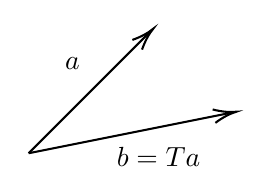
\begin{tikzpicture}[x=0.75pt,y=0.75pt,yscale=-1,xscale=1]
%uncomment if require: \path (0,94); %set diagram left start at 0, and has height of 94

%Straight Lines [id:da5287684001994821] 
\draw    (260,70) -- (318.59,11.41) ;
\draw [shift={(320,10)}, rotate = 495] [color={rgb, 255:red, 0; green, 0; blue, 0 }  ][line width=0.75]    (10.93,-3.29) .. controls (6.95,-1.4) and (3.31,-0.3) .. (0,0) .. controls (3.31,0.3) and (6.95,1.4) .. (10.93,3.29)   ;
%Straight Lines [id:da7848285394729484] 
\draw    (260,70) -- (358.04,50.39) ;
\draw [shift={(360,50)}, rotate = 528.69] [color={rgb, 255:red, 0; green, 0; blue, 0 }  ][line width=0.75]    (10.93,-3.29) .. controls (6.95,-1.4) and (3.31,-0.3) .. (0,0) .. controls (3.31,0.3) and (6.95,1.4) .. (10.93,3.29)   ;

% Text Node
\draw (276,22.4) node [anchor=north west][inner sep=0.75pt]    {$\vt{a}$};
% Text Node
\draw (301,65.4) node [anchor=north west][inner sep=0.75pt]    {$\vt{b}=\ts{T}\vt{a}$};

\end{tikzpicture}